% File: jupiter-css-c3o3-s123.tex
% CSS lattice for jupiter-scheduling-c3o3.tex

\documentclass{standalone}

% preamble for jupiter-paper related TikZ drawing
\usepackage{tikz}
\usetikzlibrary{shapes, positioning, arrows.meta, calc, backgrounds, fit}

% default horizontal/vertical distance
\def\hdist{1.5}
\def\vdist{1.5}

\newcommand{\state}[2]{% #1: state label; #2: position
  \node (#1) [circle, inner sep = 0pt, minimum size = 10mm, text width = 10mm, align = center, draw, thick, #2, font = \Large] {$#1$};
}

\newcommand{\transition}[4][]{% #2: start state; #3: end state; #4: transition label; #1: transition label position (optional)
  \draw[>=Stealth, ->, thick] (#2) to node [rectangle, draw, above = 2pt, sloped, #1, thick] {#4} (#3);
}

\tikzset{node distance = \vdist and \hdist}
\tikzset{path/.style = {draw, rounded corners, very thick, #1}}

\newcommand{\trans}[4]{% #1: start state; #2: end state; #3: transition label; #4: transition label style
  \draw[>=Stealth, ->, ultra thick, red] (#1) to node [rectangle, draw, above = 2pt, sloped, #4] {#3} (#2);
}

\begin{document}
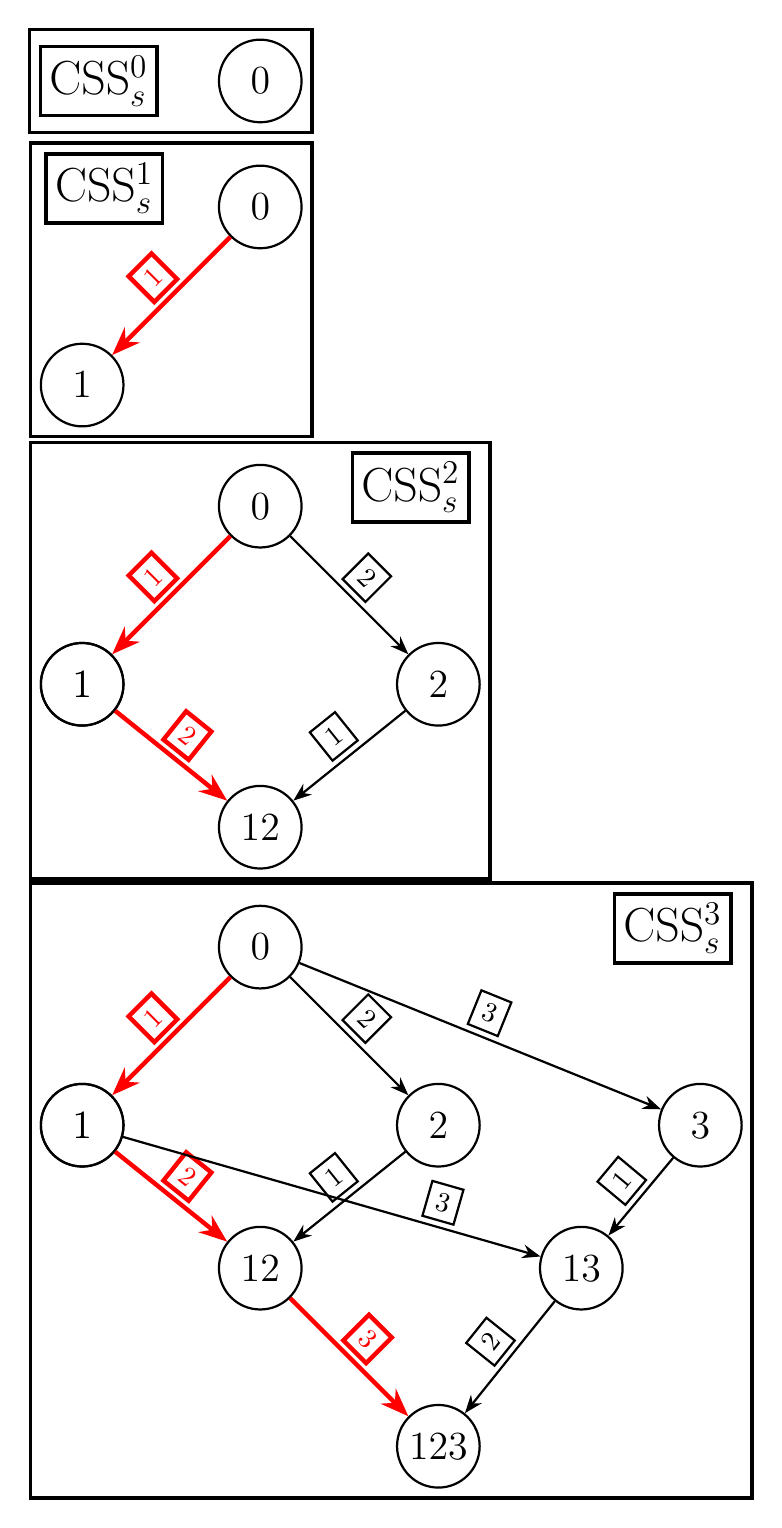
\begin{tikzpicture}[css/.style = {font = \LARGE, rectangle, draw, very thick},
	bg/.style = {rectangle, draw, very thick}]
  \begin{scope}
	\state{0}{}

	\begin{pgfonlayer}{background}
	  \node (ss) [css, left = of 0.center, xshift = 6pt] {CSS$_{s}^{0}$};
	  \node () [fit = (0) (ss), bg] {};
	\end{pgfonlayer}
  \end{scope}

  \begin{scope}[yshift = -1.6cm]
	\state{0}{}
	\state{1}{below left = of 0}
	\trans{0}{1}{1}{}
    % \transition{0}{1}{1}

	\begin{pgfonlayer}{background}
	  \node (ss) [css, above = of 1, xshift = 8pt] {CSS$_{s}^{1}$};
	  \node () [fit = (0) (1) (ss), bg] {};
	\end{pgfonlayer}
  \end{scope}

  \begin{scope}[yshift = -5.4cm]
    \state{0}{}
    \state{1}{below left = of 0}
    \state{1}{below left = of 0}
    \state{2}{below right = of 0}
    \state{12}{below = 2*\vdist of 0}
	\trans{0}{1}{1}{}
    % \transition{0}{1}{1}
    \transition{0}{2}{2}
	\trans{1}{12}{2}{}
    % \transition{1}{12}{2}
    \transition{2}{12}{1}

	\begin{pgfonlayer}{background}
	  \node (ss) [css, above = of 2, xshift = -10pt] {CSS$_{s}^{2}$};
	  \node () [fit = (0) (1) (2) (12) (ss), bg] {};
	\end{pgfonlayer}
  \end{scope}

  \begin{scope}[shift = {(0, -11)}]
    \state{0}{}
    \state{1}{below left = of 0}
    \state{1}{below left = of 0}
    \state{2}{below right = of 0}
    \state{12}{below = 2*\vdist of 0}
	\trans{0}{1}{1}{}
    % \transition{0}{1}{1}
    \transition{0}{2}{2}
	\trans{1}{12}{2}{}
    % \transition{1}{12}{2}
    \transition{2}{12}{1}
    \state{3}{right = 1.5*\vdist of 2}
    \transition{0}{3}{3}
    \state{13}{right = 2*\hdist of 12}
    \transition[near end]{1}{13}{3}
    \transition{3}{13}{1}

    \state{123}{below = 2*\vdist of 2}
	\trans{12}{123}{3}{}
    % \transition{12}{123}{3}
    \transition{13}{123}{2}

	\begin{pgfonlayer}{background}
	  \node (ss) [css, above = of 3, xshift = -10pt] {CSS$_{s}^{3}$};
	  \node () [fit = (0) (1) (3) (123) (ss), bg] {};
	\end{pgfonlayer}
  \end{scope}
\end{tikzpicture}
\end{document}
